\documentclass[12pt,pdf,hyperref={unicode}]{beamer}


%\documentclass[10pt]{beamer}

\usetheme[progressbar=frametitle]{metropolis}

\usepackage{booktabs}
\usepackage[scale=2]{ccicons}

\usepackage{pgfplots}
\usepgfplotslibrary{dateplot}

\usepackage{xspace}
\newcommand{\themename}{\textbf{\textsc{metropolis}}\xspace}

%\usepackage{lmodern}

% подключаем кириллицу 
\usepackage[T2A]{fontenc}
\usepackage[utf8]{inputenc}
\usepackage{listings}
%\usepackage{graphicx}
\usepackage{hyperref}

% отключить клавиши навигации
\setbeamertemplate{navigation symbols}{}

% тема оформления
\usetheme{Pittsburgh}

% цветовая схема
\usecolortheme{default}

\definecolor{light-gray}{gray}{0.90}

\title{Семинар №5}   
\subtitle{ФАКИ \the\year}
\author{Бирюков В. А.} 
\date{\today} 
% \logo{
\includegraphics[height=5mm]{images/logo.png}\vspace{-7pt}}

\begin{document}

\lstset{language=C}

% титульный слайд
\begin{frame}
\titlepage
\end{frame} 

\defverbatim[colored]\makeset{
\begin{lstlisting}[language=C++,basicstyle=\ttfamily,keywordstyle=\color{blue}]
void make_set(int X) {
  parent[X] = X;
}
\end{lstlisting}
}

\lstset{
  language=C,                % choose the language of the code
  keywordstyle=\color{blue},
  numbers=none,                   % where to put the line-numbers
  stepnumber=1,                   % the step between two line-numbers.        
  numbersep=5pt,                  % how far the line-numbers are from the code
  backgroundcolor=\color{white!90!gray},  % choose the background color. You must add \usepackage{color}
  showspaces=false,               % show spaces adding particular underscores
  showstringspaces=false,         % underline spaces within strings
  showtabs=false,                 % show tabs within strings adding particular underscores
  tabsize=2,                      % sets default tabsize to 2 spaces
  captionpos=b,                   % sets the caption-position to bottom
  breaklines=true,                % sets automatic line breaking
  breakatwhitespace=true,         % sets if automatic breaks should only happen at whitespace
}

\section{Кодировки. Символы. Тип char}

\begin{frame}[fragile]
\frametitle{Кодировки} 
Кодировка -- таблица в которой символам сопоставлены числовые коды.
\begin{itemize}
\item ASCII (American standard code for information interchange) -- разработана в 1963 году, 7 битовая -- можно закодировать 128 символов, но занимает 1 байт.
\item Unicode (UTF-8, UTF-16, UTF-32) -- можно закодировать 1112064 различных символов. UTF-8 -- самая распространённая кодировка, символ занимает от 1 до 4 байт.
\end{itemize}
\end{frame}


\begin{frame}[fragile]
\frametitle{Символы} 
\textbf{char} -- тип данных, предназначенный для хранения одного символа в кодировке ASCII. Представляет собой целочисленный тип. Диапазон от -128 до 127 (или от 0 до 255).
\begin{lstlisting}
char a = 105;
char b = 'N';
printf("%c\n", '+');
\end{lstlisting}
\end{frame}


\begin{frame}[fragile]
\begin{center}
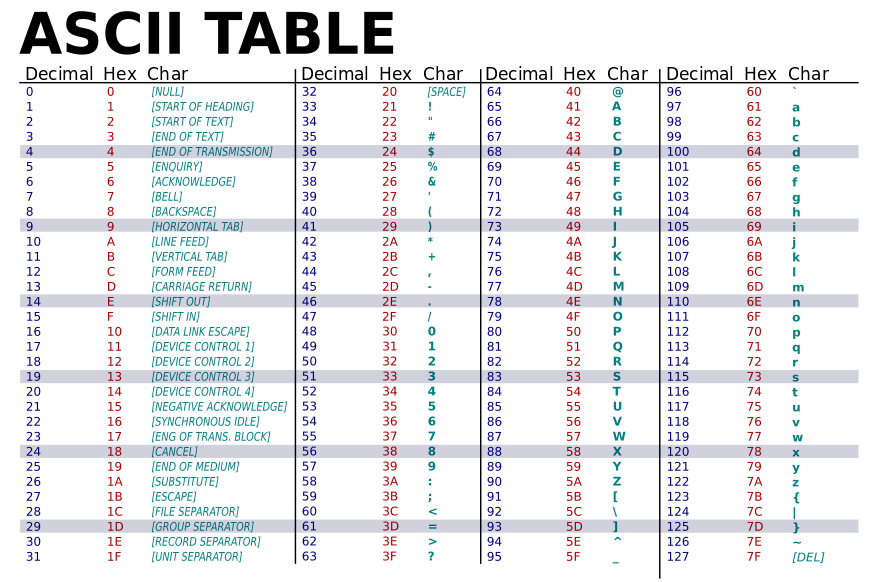
\includegraphics[width=1.05\linewidth]{images/ascii.png}
\end{center}
\end{frame}

\begin{frame}[fragile]
\frametitle{Символы}
\begin{center}
\begin{tabular}{ c | c | c }
  {\color{red}\textbf{'0'}} = 48 & {\color{red}\textbf{'A'}} = 65 & нулевой символ  {\color{red}\textbf{'\textbackslash 0'}} = 0 \\
  {\color{red}\textbf{'1'}} = 49 & {\color{red}\textbf{'B'}} = 66 & символ переноса строки {\color{red}\textbf{'\textbackslash n'}} = 10 \\
  {\color{red}\textbf{'2'}} = 50 & ...                             & табуляция {\color{red}\textbf{'\textbackslash t'}} = 9 \\
  ...                            & {\color{red}\textbf{'Z'}} = 90 & backspace {\color{red}\textbf{'\textbackslash b'}} = 8 \\
  {\color{red}\textbf{'9'}} = 57 & {\color{red}\textbf{'a'}} = 97 & звуковой сигнал {\color{red}\textbf{'\textbackslash a'}} = 7 \\
  {\color{red}\textbf{' '}} = 32 & ...                           & возврат каретки {\color{red}\textbf{'\textbackslash r'}} = 13 \\
                                 & {\color{red}\textbf{'z'}} = 122  &   \\
\end{tabular}
\end{center}
\end{frame}


\section{Строки}

\begin{frame}[fragile]
\frametitle{Строки} 
\begin{itemize}
\item Строки в языке C -- на самом деле массивы из элементов типа char
\item В конце строки должен стоять символ '\textbackslash 0'
\item Объявление:
\begin{lstlisting}
char s[10];
\end{lstlisting}
\item Доступ к элементу
(Нумерация в строке тоже начинается с 0):\\
\begin{lstlisting}
printf("%c\n", s[0]);
\end{lstlisting}
\end{itemize}
\end{frame}


\begin{frame}[fragile]
\frametitle{Строки} 
\framesubtitle{Инициализация}
\begin{lstlisting}
char hello_str[10] = {'h', 'e', 'l', 'l', 'o', '\0'};
\end{lstlisting}
\begin{lstlisting}
char hello_str[10] = "hello";
\end{lstlisting}
Во втором случае нулевой символ задаётся автоматически
\end{frame}

\begin{frame}[fragile]
\frametitle{Строки} 
\framesubtitle{Строки в памяти}
\begin{center}
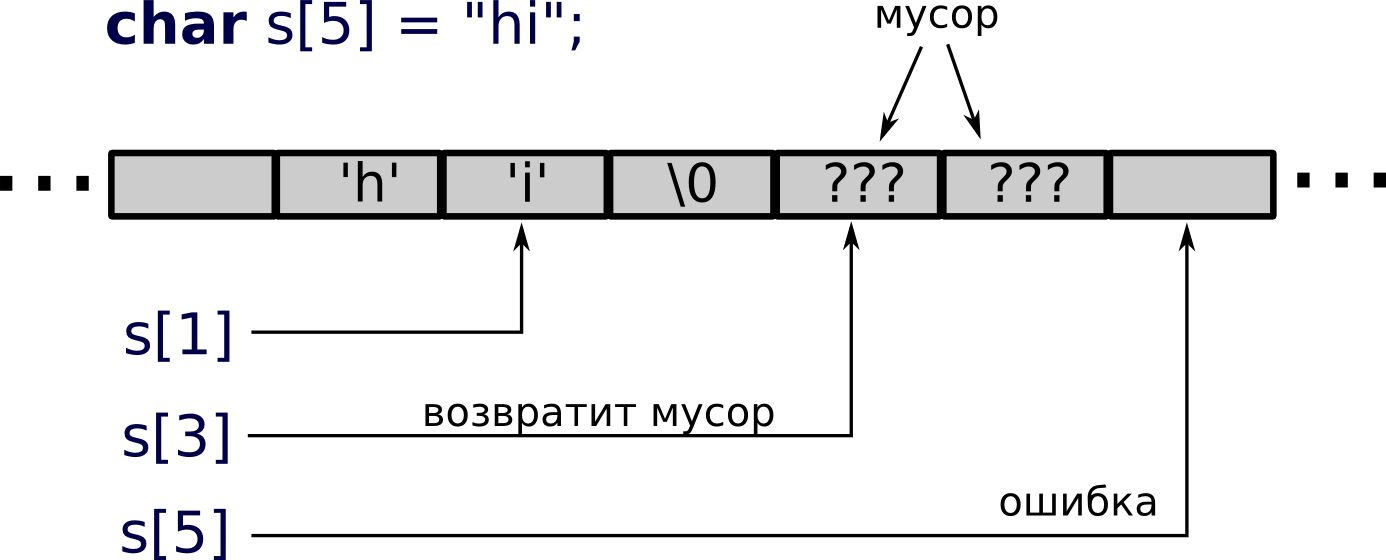
\includegraphics[width=0.95\linewidth]{images/string_in_memory.png}
\end{center}
\end{frame}

\begin{frame}[fragile]
\frametitle{Строки} 
\framesubtitle{Дополнительно}
Чтение строки:
\begin{lstlisting}
char string[10];
scanf("%s", string);
\end{lstlisting}
Cчитывание из строки (функция sscanf()):
\begin{lstlisting}
int string[10] = "15:20";
int h, m;
sscanf(string, "%d:%d", &h, &m);
\end{lstlisting}
Можно использовать для конвертирования строки в число.
\end{frame}

\section{Функции для работы со строками (библиотека string.h)}

\begin{frame}[fragile]
\frametitle{Функция strlen} 
\begin{lstlisting}
size_t strlen(const char*);
\end{lstlisting}
возвращает длину строки (size\_t -- беззнаковый целый тип)
\begin{lstlisting}
#include <string.h>
int string[10] = "hello";
int n = strlen(string);
\end{lstlisting}
В этом примере n будет равно 5.
\end{frame}


\begin{frame}[fragile]
\frametitle{Функция strcpy и strstr} 
\begin{lstlisting}
char* strcpy(char* dest, const char* src);
\end{lstlisting}
Функция strcpy копирует строку из исходной строки src в строку dest побайтово. Строка dest должна быть достаточного размера.
\iffalse
\begin{lstlisting}
char* strcat(char* dest, const char* src);
\end{lstlisting}
Функция strcat дописывает содержимое исходной строки src к строке dest побайтово. Строка dest должна быть достаточного размера.
\fi
\begin{lstlisting}
char* strstr(const char* str, const char* substr);
\end{lstlisting}
Функция strstr находит первое вхождение строки substr в строке str. Возвращает указатель на первый символ этого вхождения. Если такого вхожения нет, то она возвращает NULL.
\end{frame}


\begin{frame}[fragile]
\frametitle{Функция strcmp} 
\begin{lstlisting}
int strcmp(const char*, const char*);
\end{lstlisting}
лексикографическое сравнение строк (возвращает 0, если строки одинаковые, положительное, если первая строка больше, и отрицательное, если меньше).
\begin{lstlisting}
#include <string.h>
int s1[10] = "kangaroo";
int s2[10] = "kitten";
int n = strcmp(s1, s2);
\end{lstlisting}
В этом примере $n < 0$ так как строка "kangaroo" меньше строки "kitten"(потому что 'a' < 'i').
\end{frame}


\section{Поиск наибольшей общей подпоследовательности}
\begin{frame}[fragile]
\frametitle{Поиск наибольшей общей подпоследовательности} 
\framesubtitle{Longest common subsequence, LCS}
\begin{center}

\includegraphics[width=0.40\linewidth]{images/lcs1.png}
\end{center}
\end{frame}

\begin{frame}[fragile]
\frametitle{Поиск наибольшей общей подпоследовательности} 
\begin{center}

\includegraphics[width=0.40\linewidth]{images/lcs2.png}
\end{center}
Наибольшая общая подпоследовательность равна BCAB.
\end{frame}


\begin{frame}[fragile]
\frametitle{Поиск наибольшей общей подпоследовательности} 
\begin{center}

\includegraphics[width=0.40\linewidth]{images/lcs3.png}
\end{center}
\[
C(i, j) = 
\begin{cases}
    C(i-1, j-1) + 1,             & \text{если } X[i] = Y[j]\\
    max(C(i-1, j), C(i, j-1)),   & \text{иначе}
\end{cases}
\]
\end{frame}

\begin{frame}[fragile]
\frametitle{LCS} 
\begin{center}
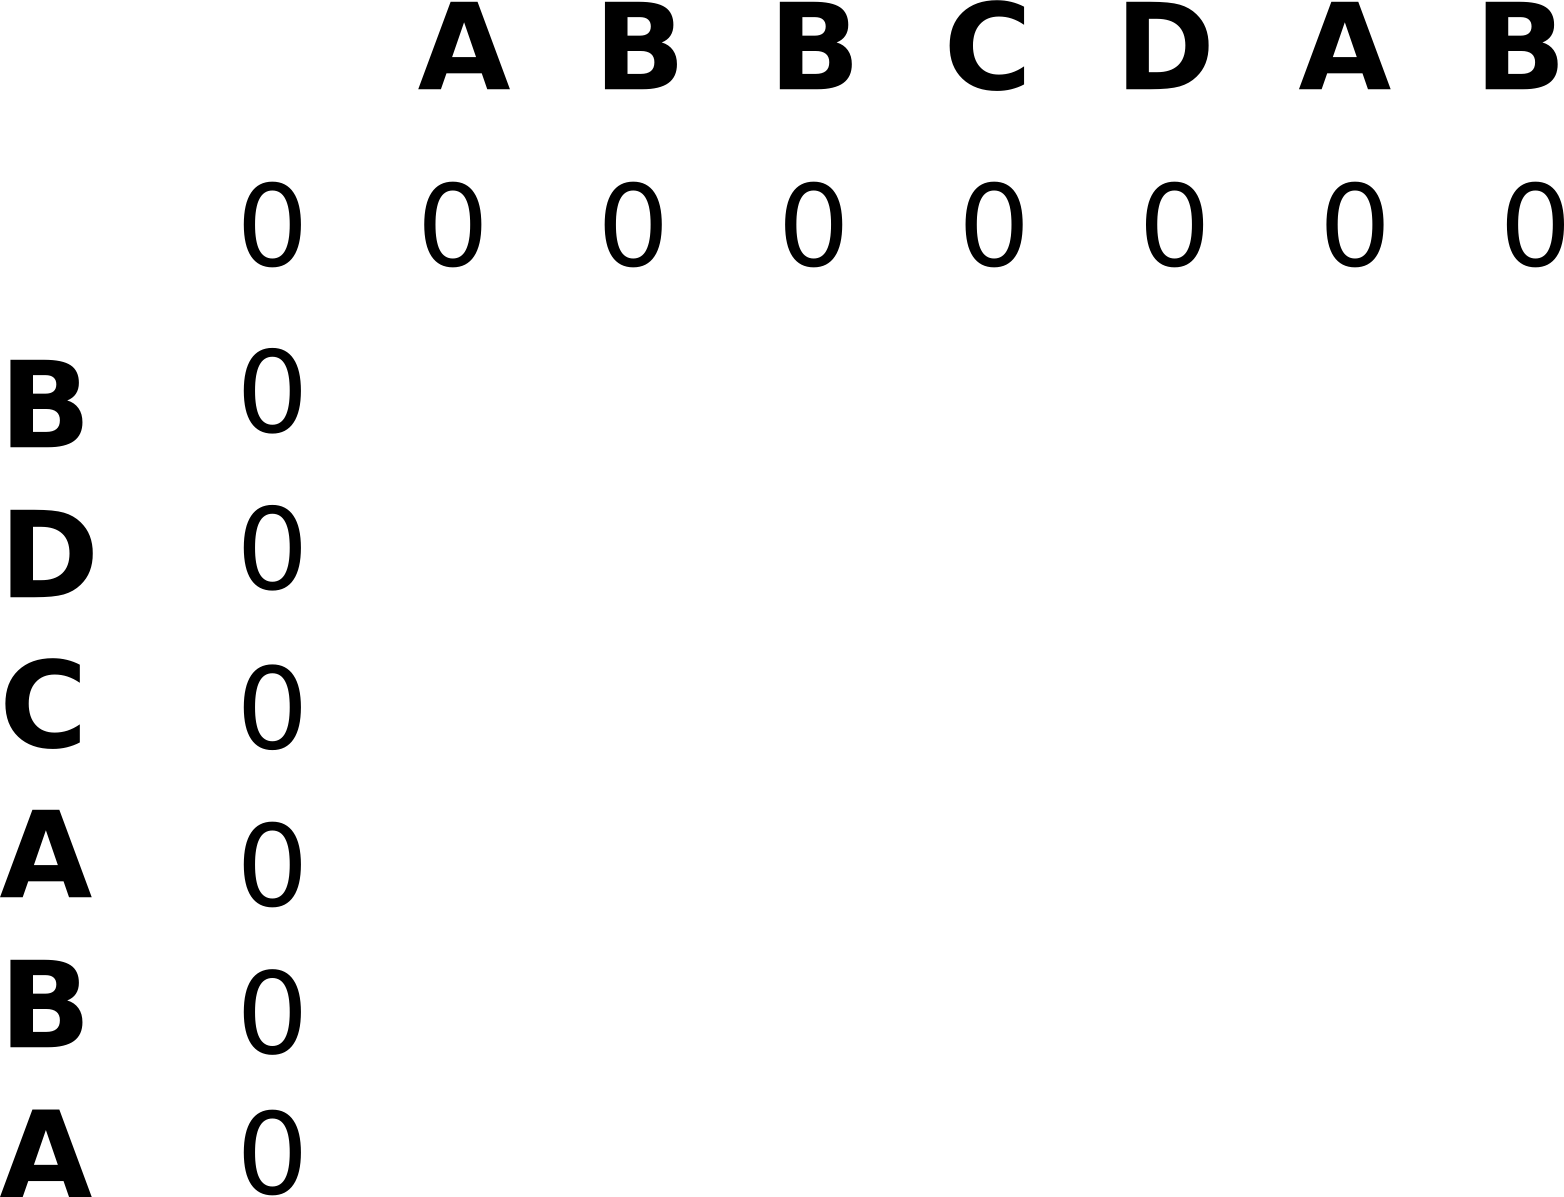
\includegraphics[width=0.75\linewidth]{images/lcstable1.png}
\end{center}
\end{frame}

\begin{frame}[fragile]
\frametitle{LCS} 
\begin{center}
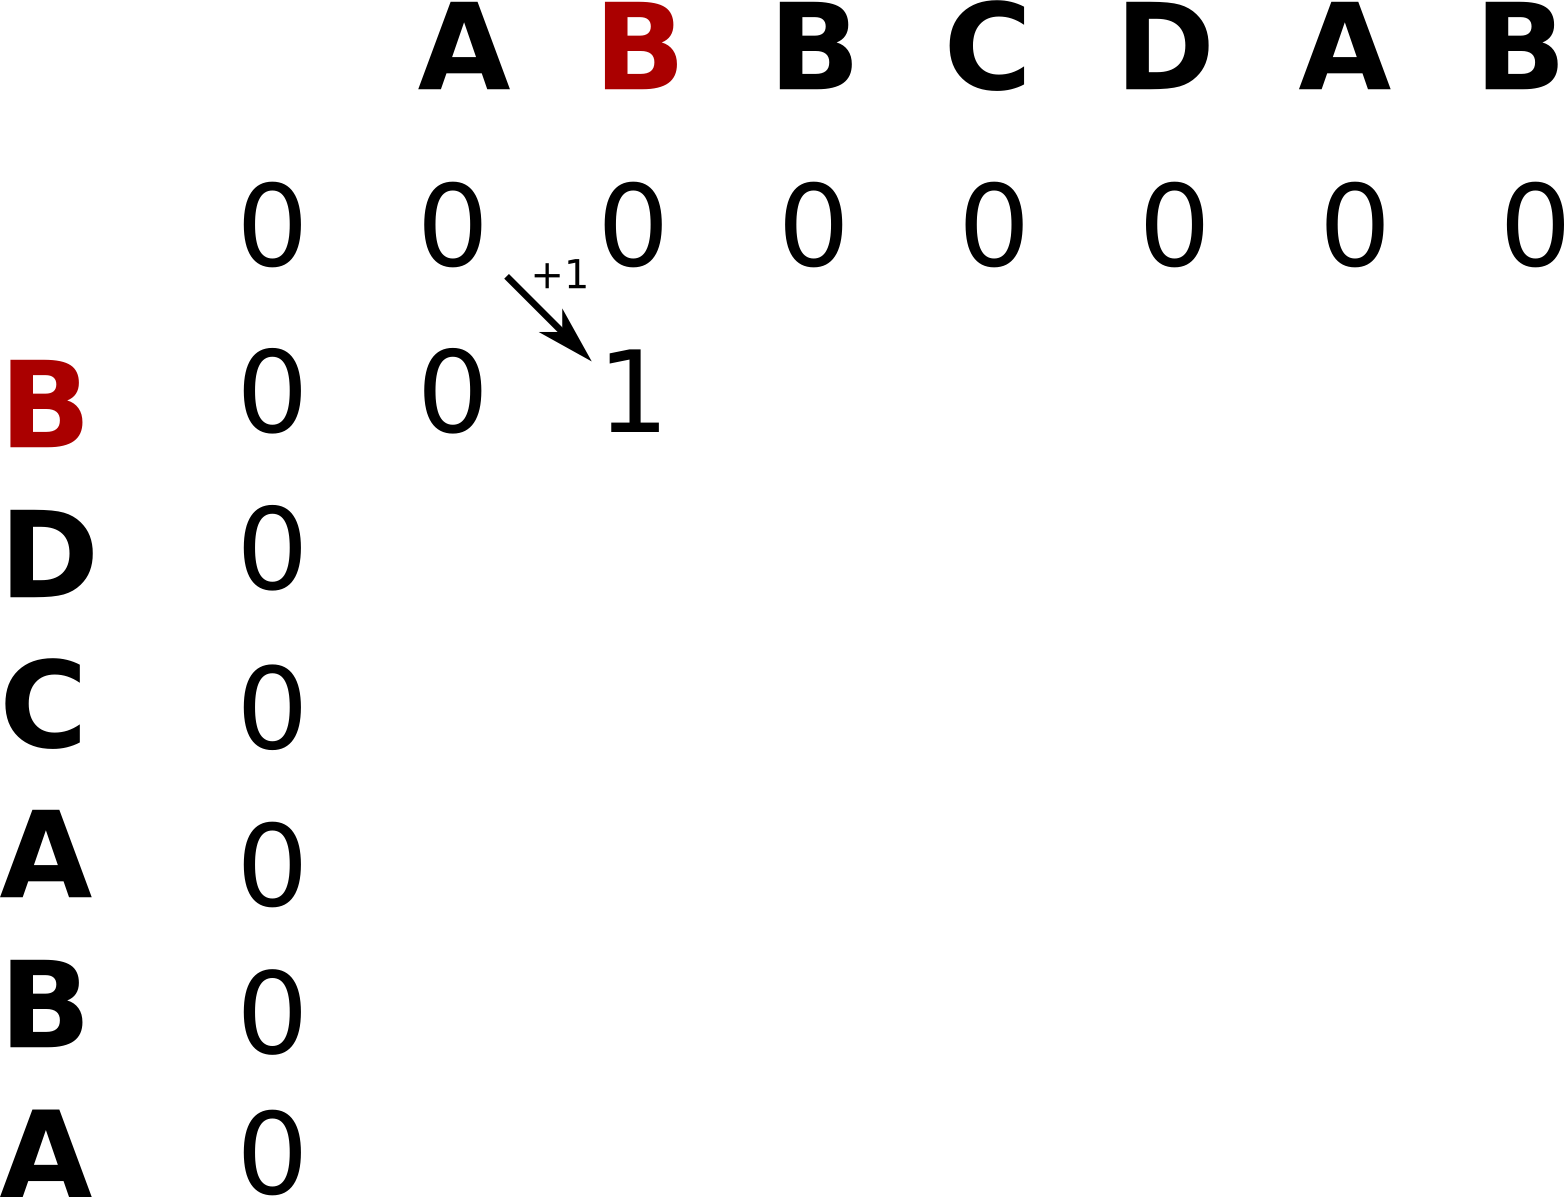
\includegraphics[width=0.75\linewidth]{images/lcstable2.png}
\end{center}
\end{frame}

\begin{frame}[fragile]
\frametitle{LCS} 
\begin{center}
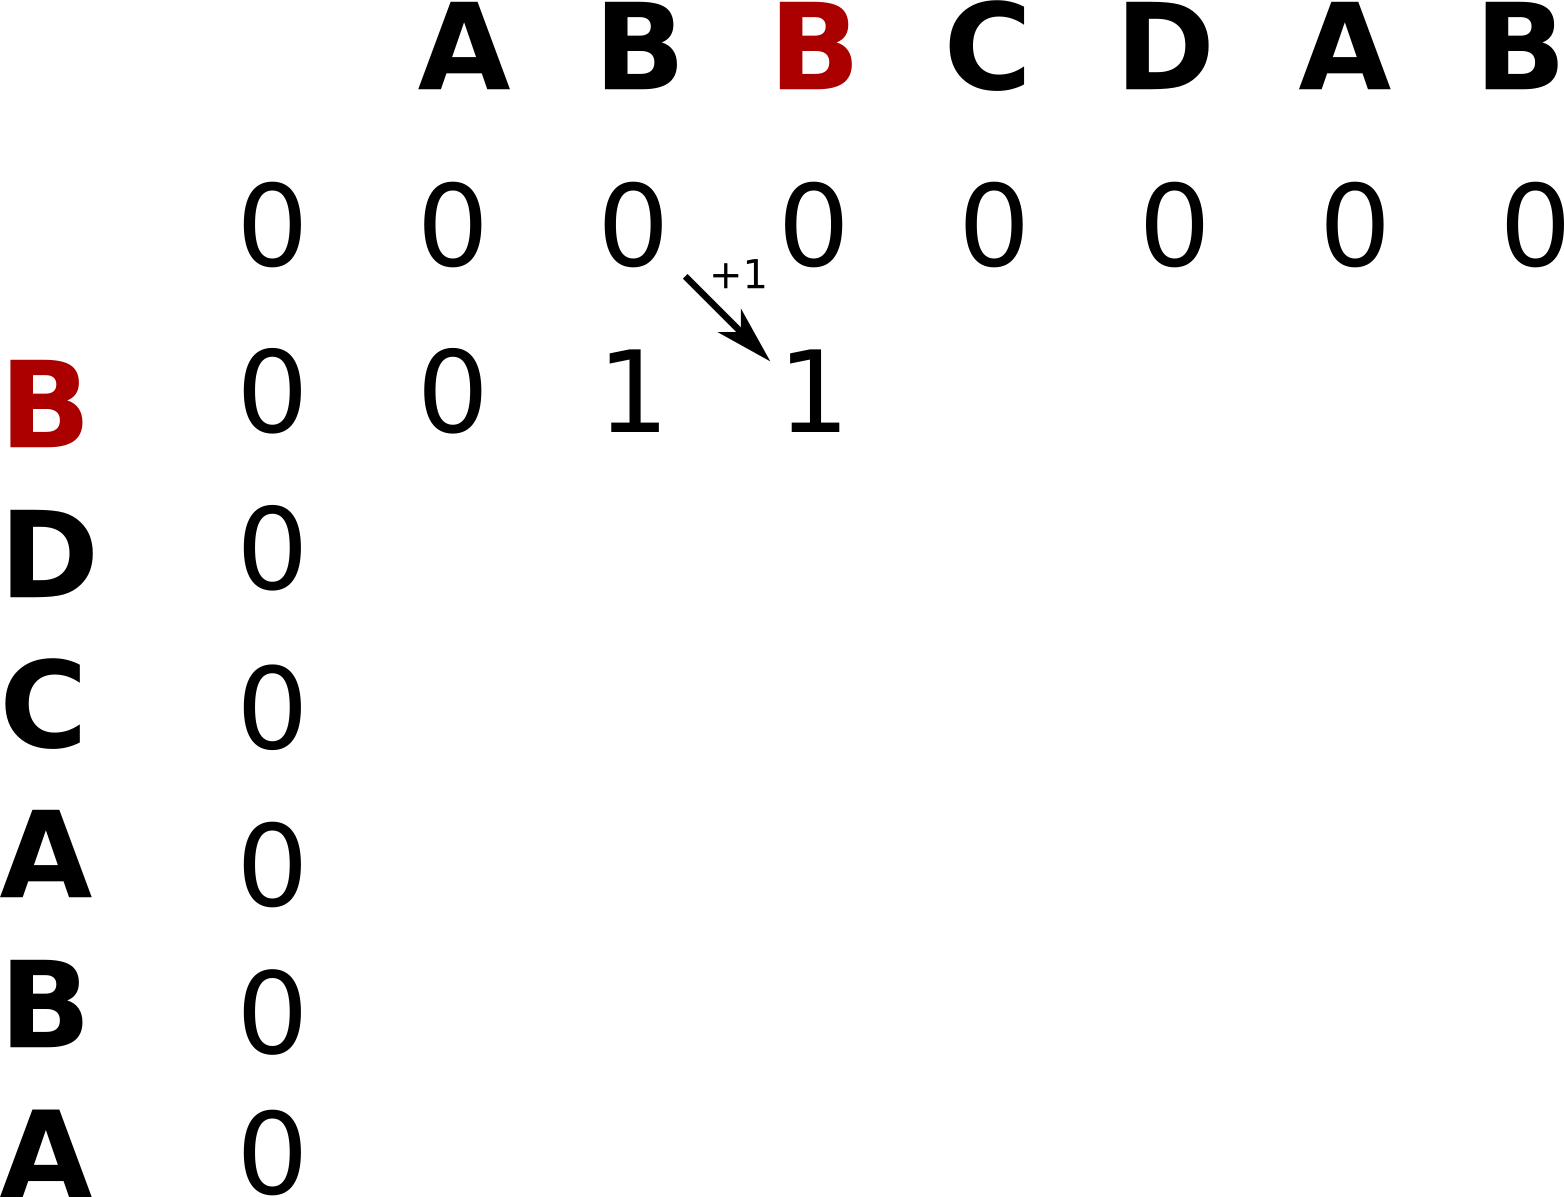
\includegraphics[width=0.75\linewidth]{images/lcstable3.png}
\end{center}
\end{frame}

\begin{frame}[fragile]
\frametitle{LCS} 
\begin{center}
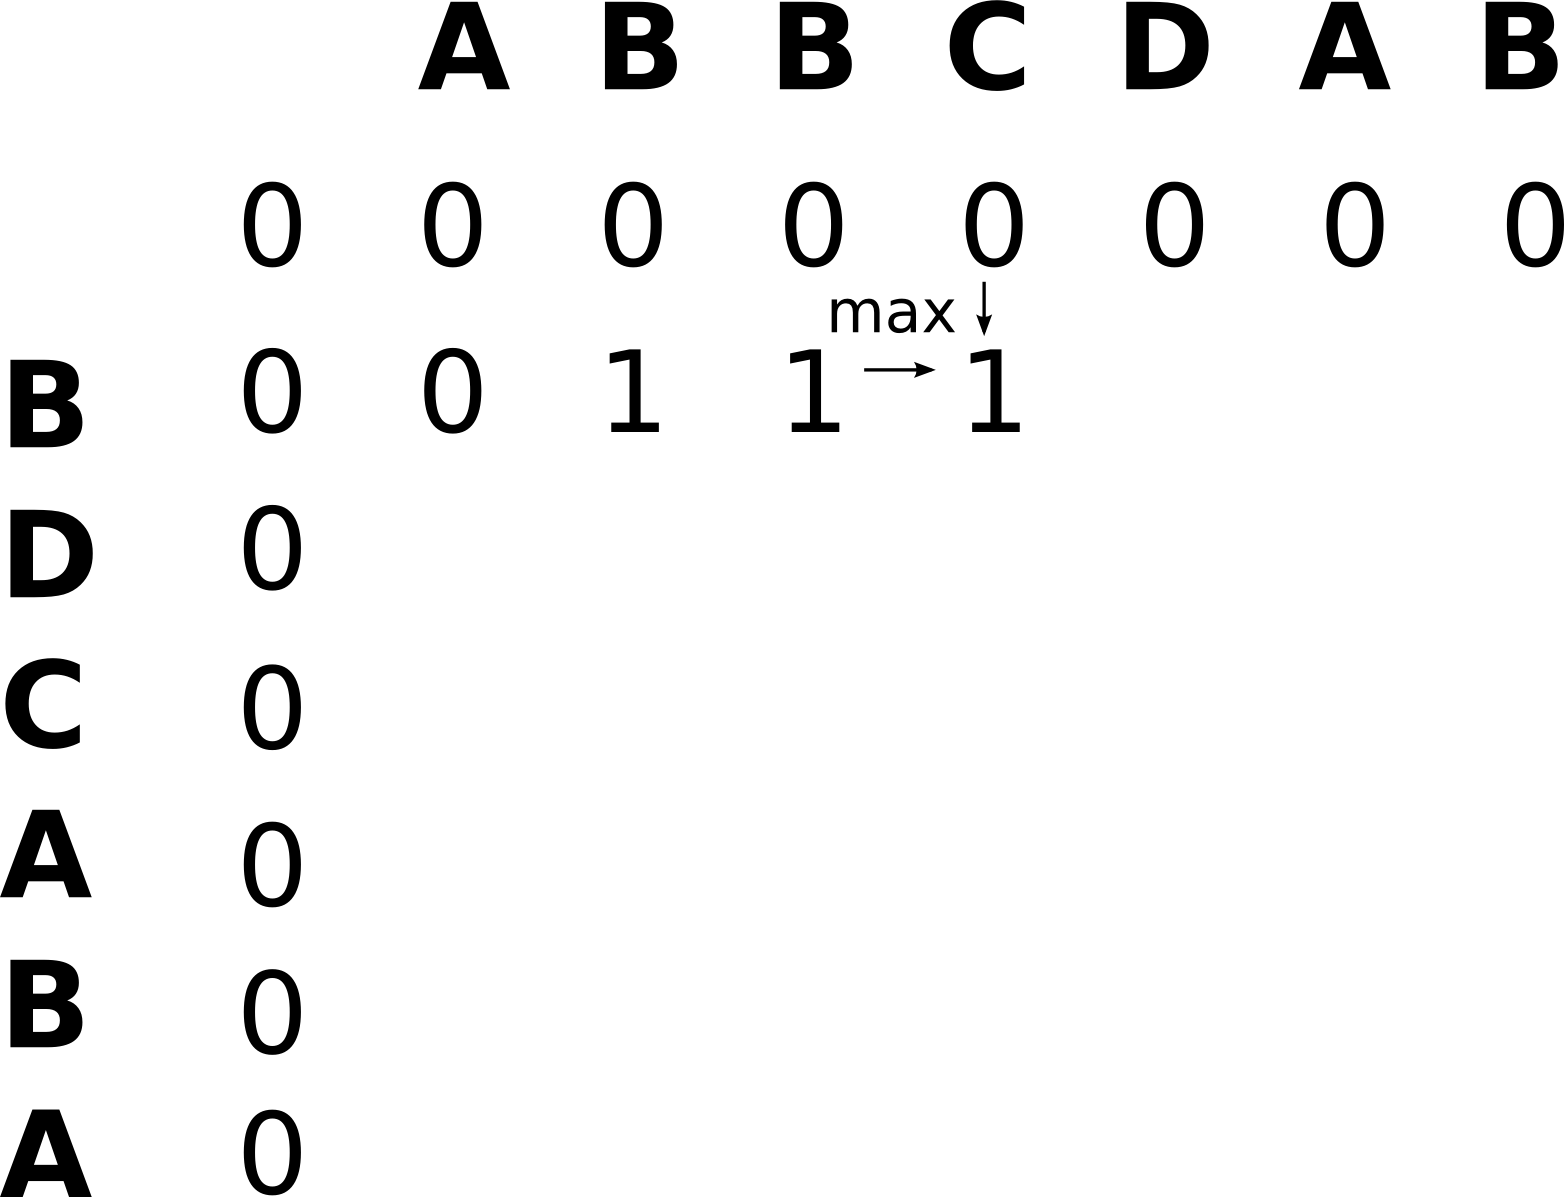
\includegraphics[width=0.75\linewidth]{images/lcstable4.png}
\end{center}
\end{frame}

\begin{frame}[fragile]
\frametitle{LCS} 
\begin{center}
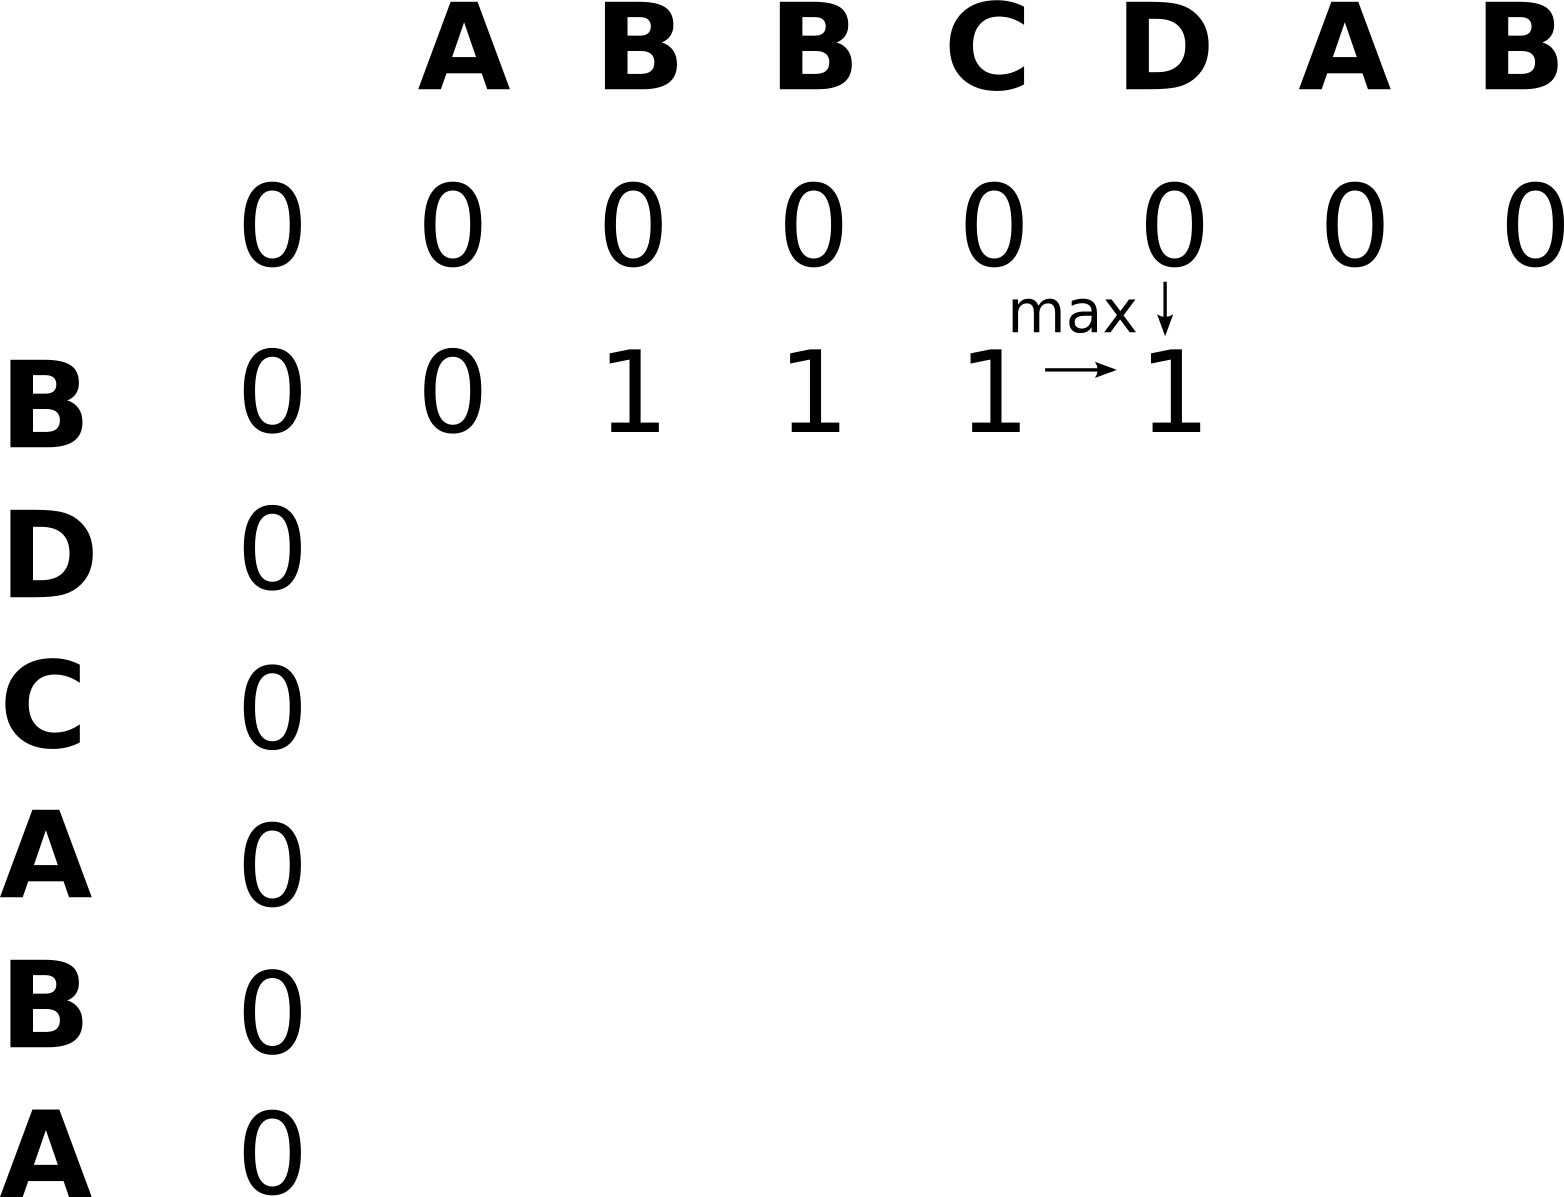
\includegraphics[width=0.75\linewidth]{images/lcstable5.png}
\end{center}
\end{frame}

\begin{frame}[fragile]
\frametitle{LCS} 
\begin{center}
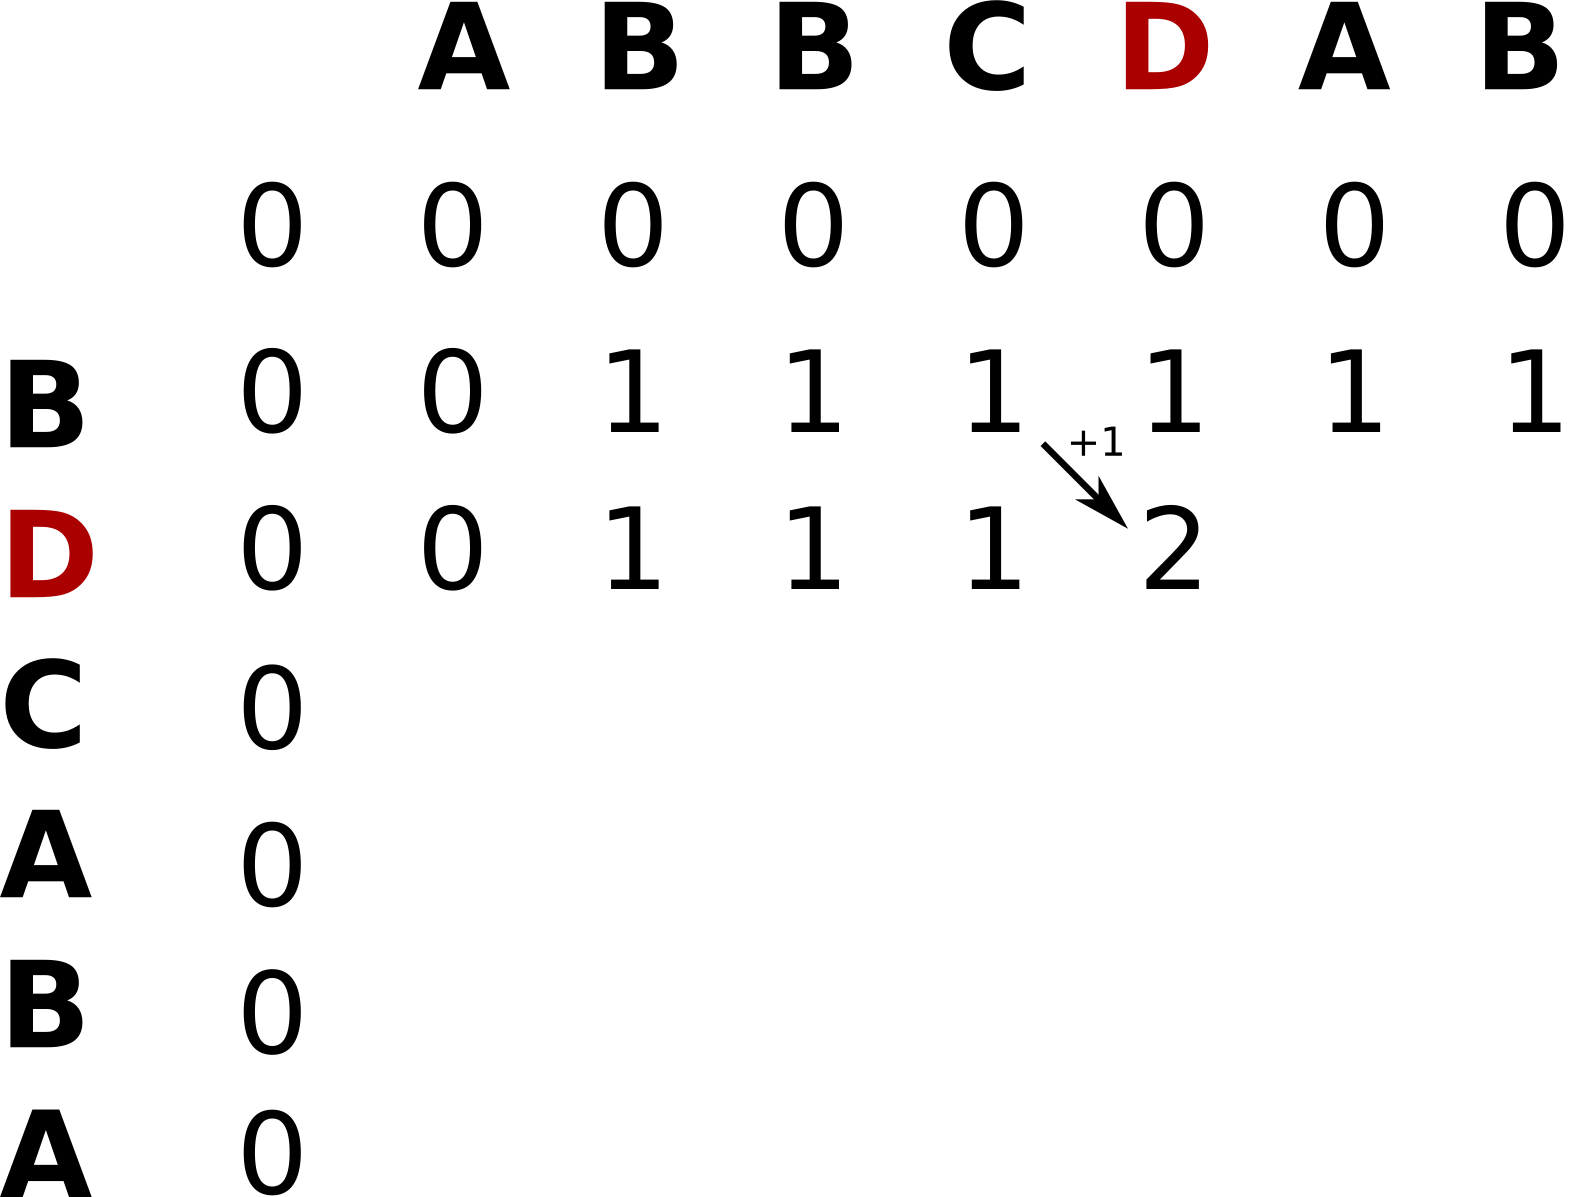
\includegraphics[width=0.75\linewidth]{images/lcstable6.png}
\end{center}
\end{frame}

\begin{frame}[fragile]
\frametitle{LCS} 
\begin{center}
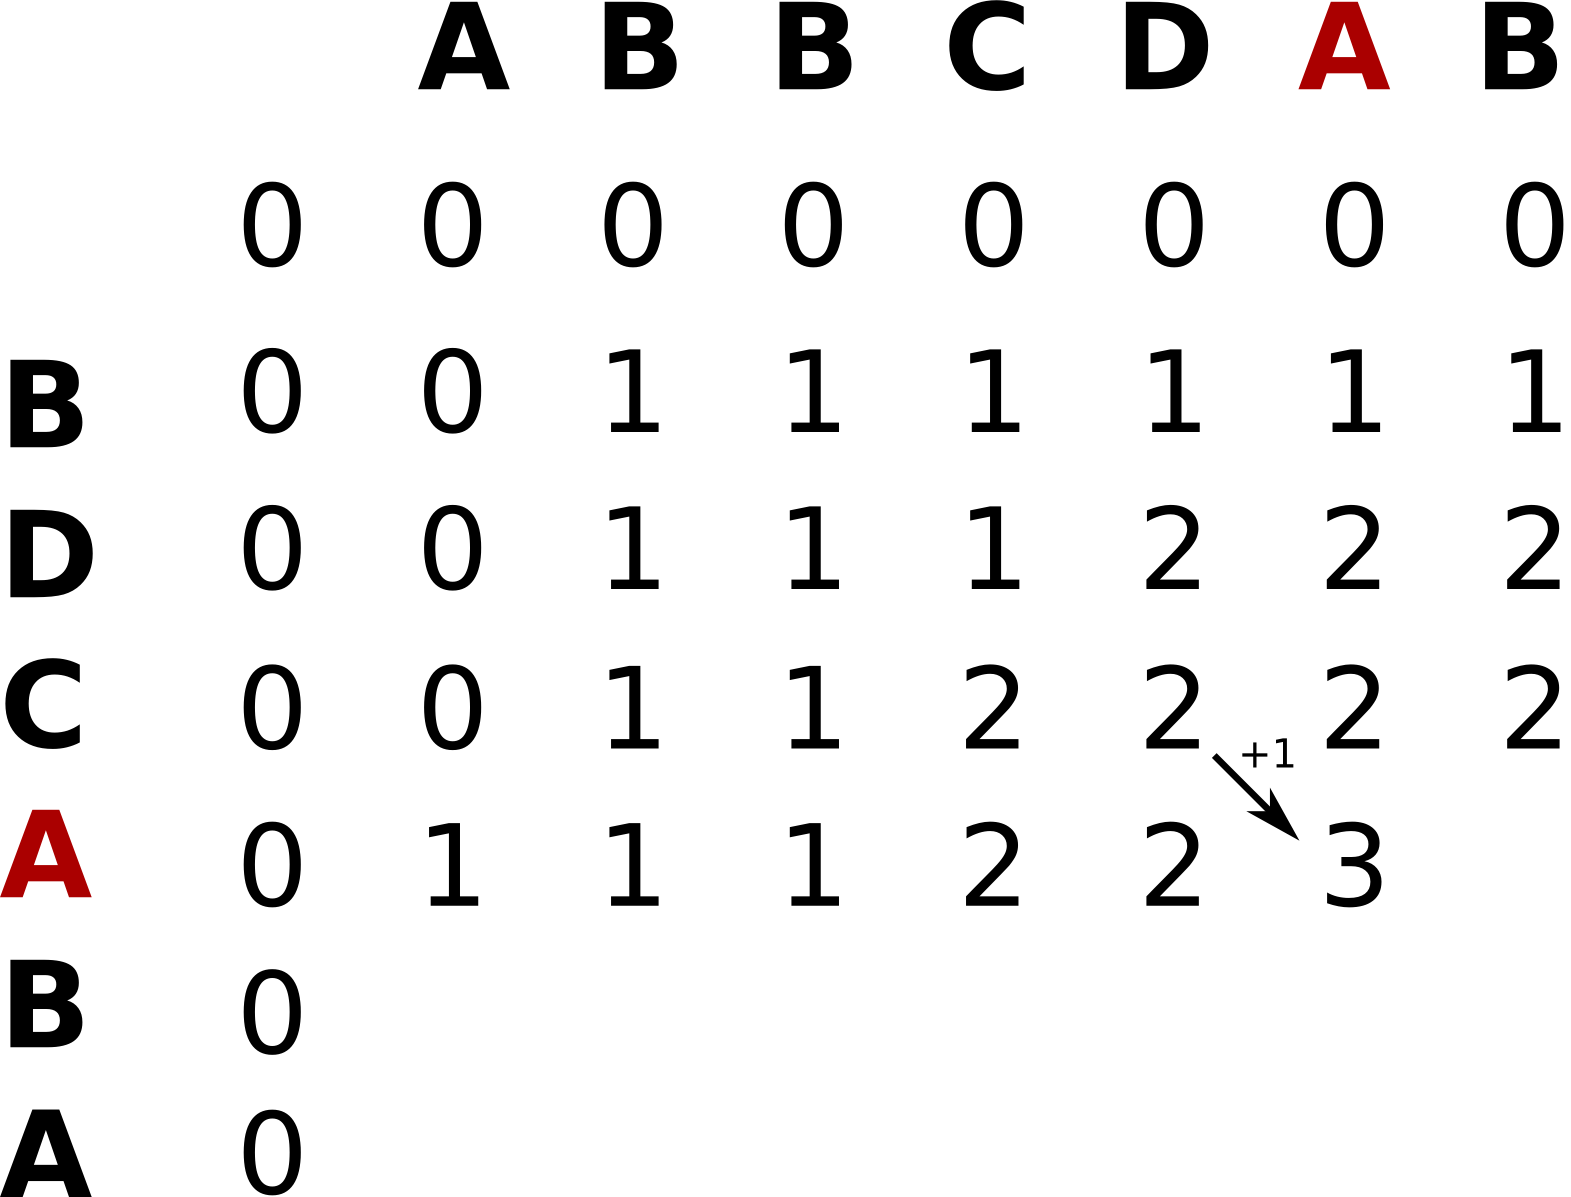
\includegraphics[width=0.75\linewidth]{images/lcstable7.png}
\end{center}
\end{frame}

\begin{frame}[fragile]
\frametitle{LCS} 
\begin{center}
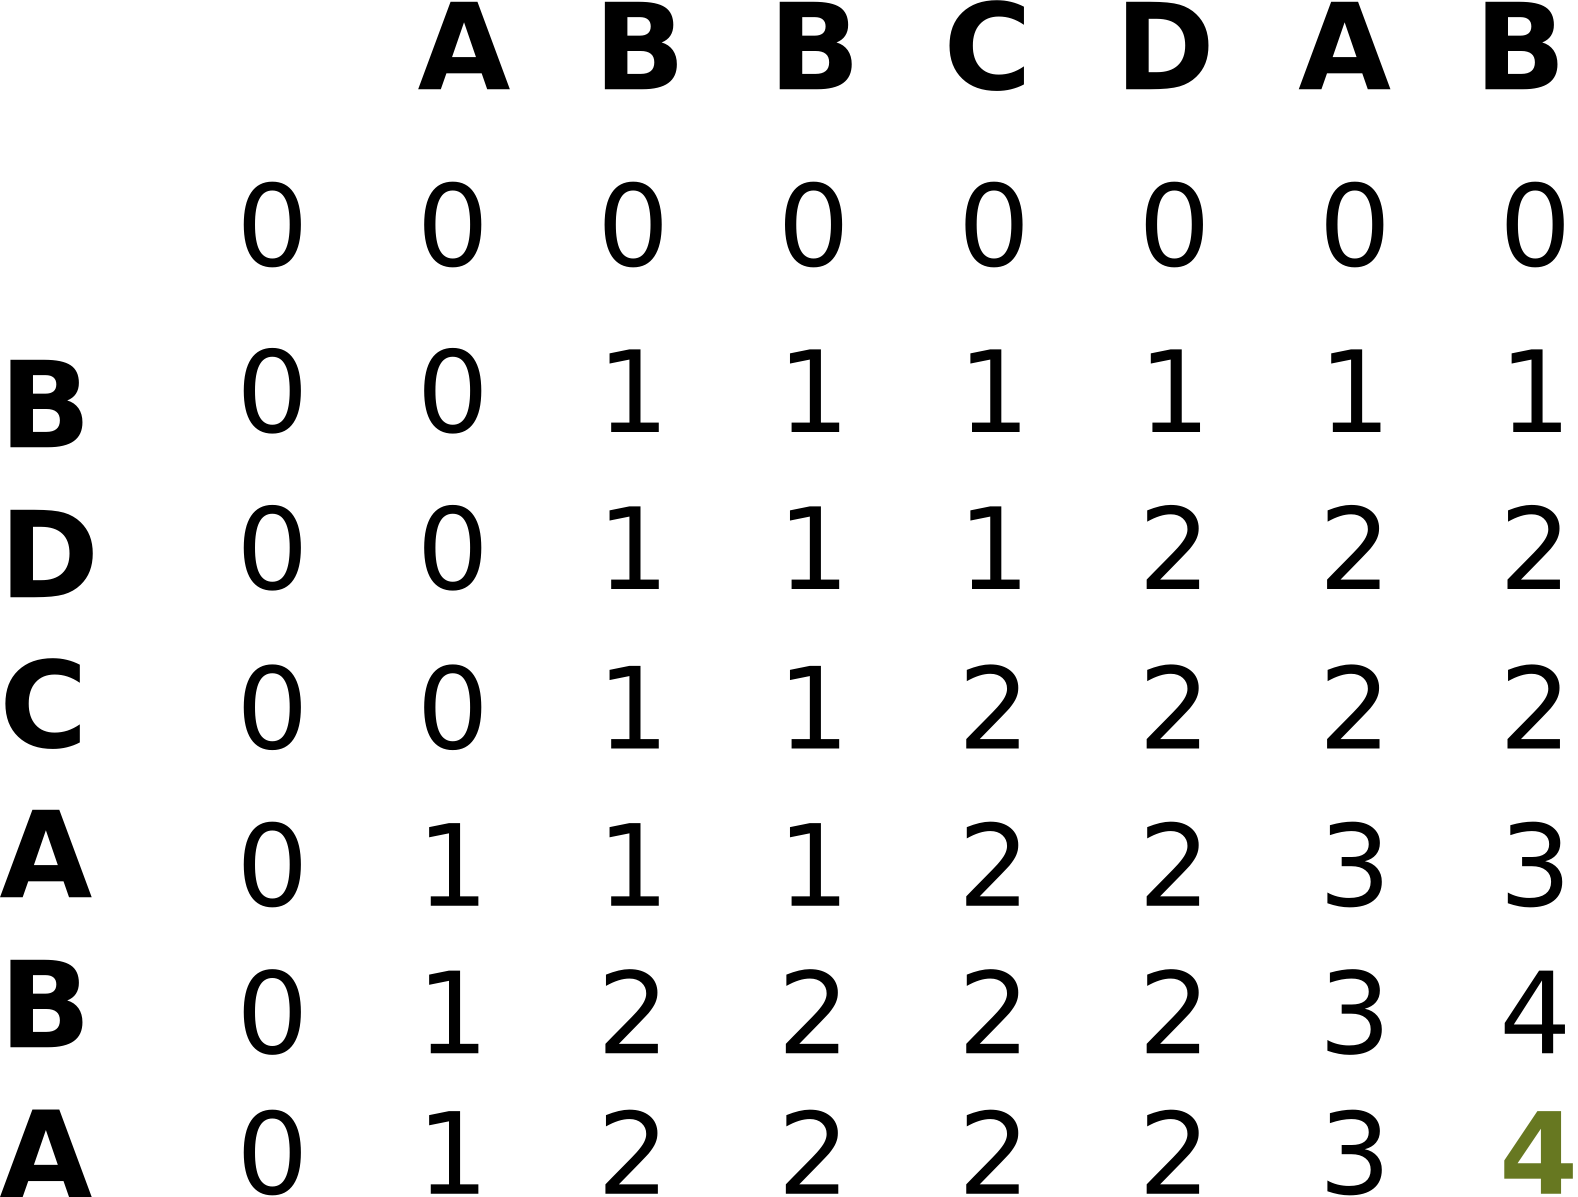
\includegraphics[width=0.75\linewidth]{images/lcstable8.png}
\end{center}
\end{frame}

\begin{frame}[fragile]
\frametitle{LCS} 
\begin{center}
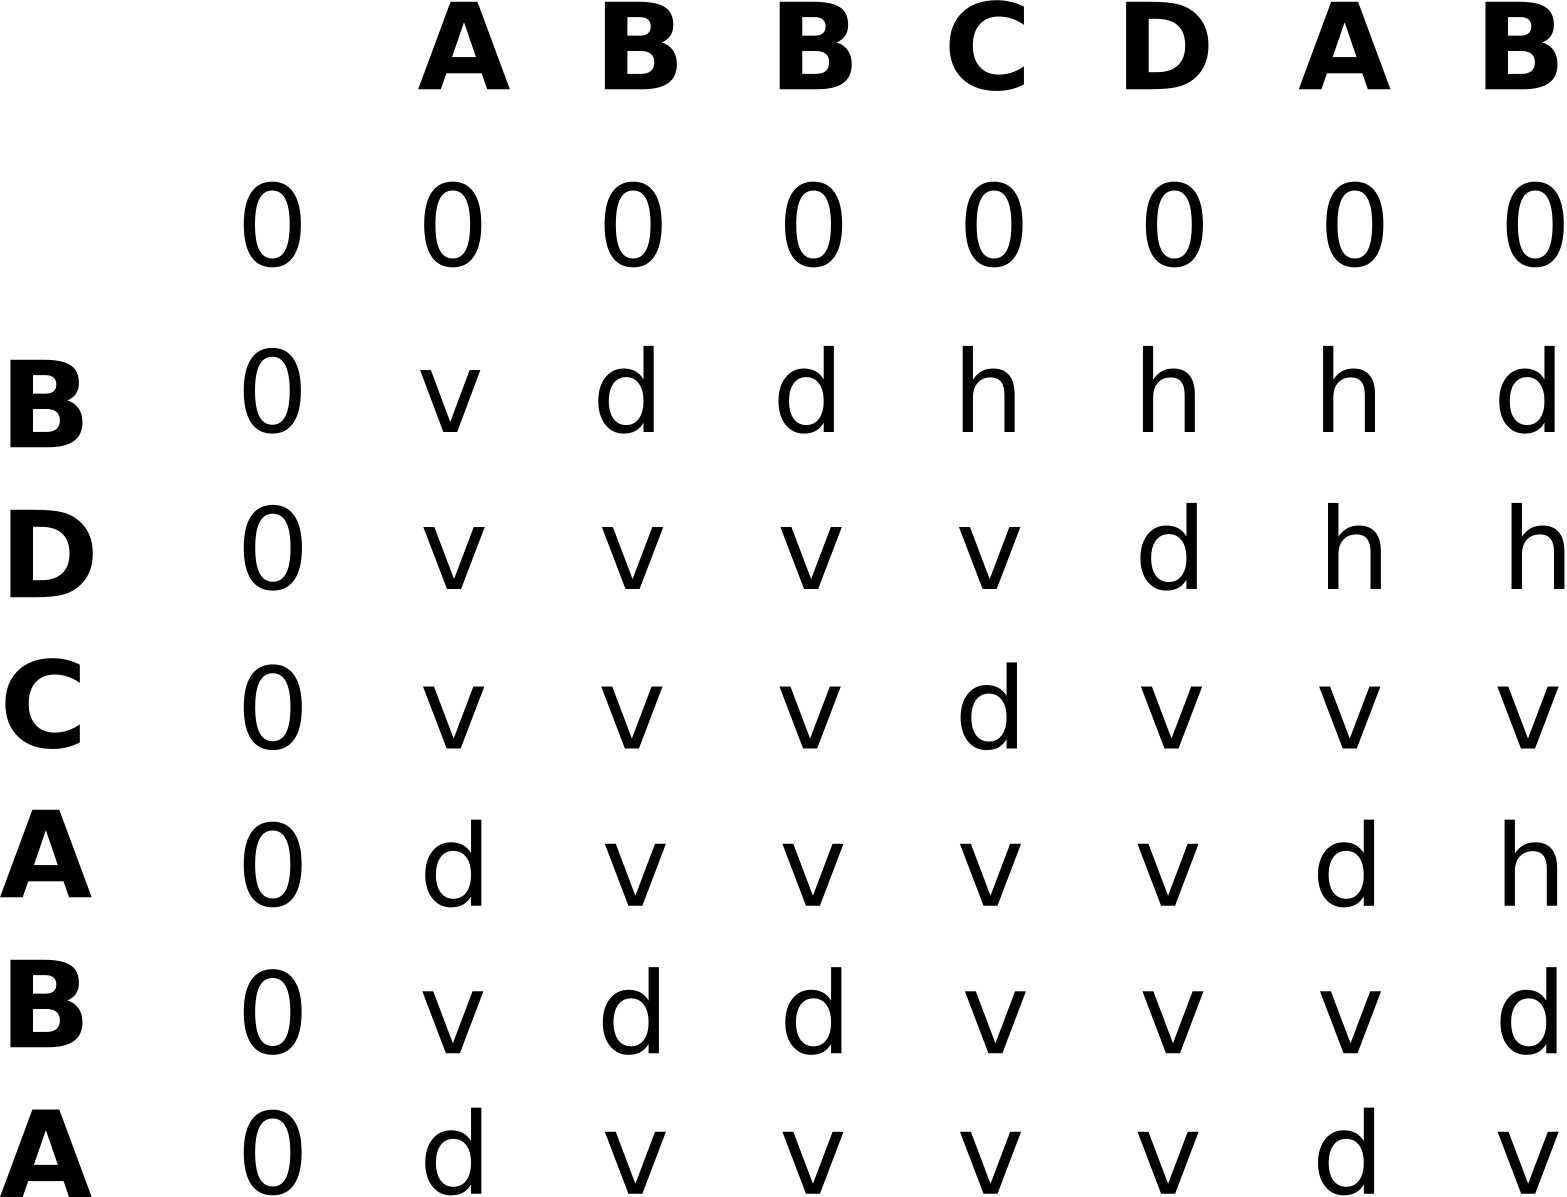
\includegraphics[width=0.75\linewidth]{images/lcstable9.png}
\end{center}
\end{frame}

\begin{frame}[fragile]
\frametitle{LCS} 
\begin{center}
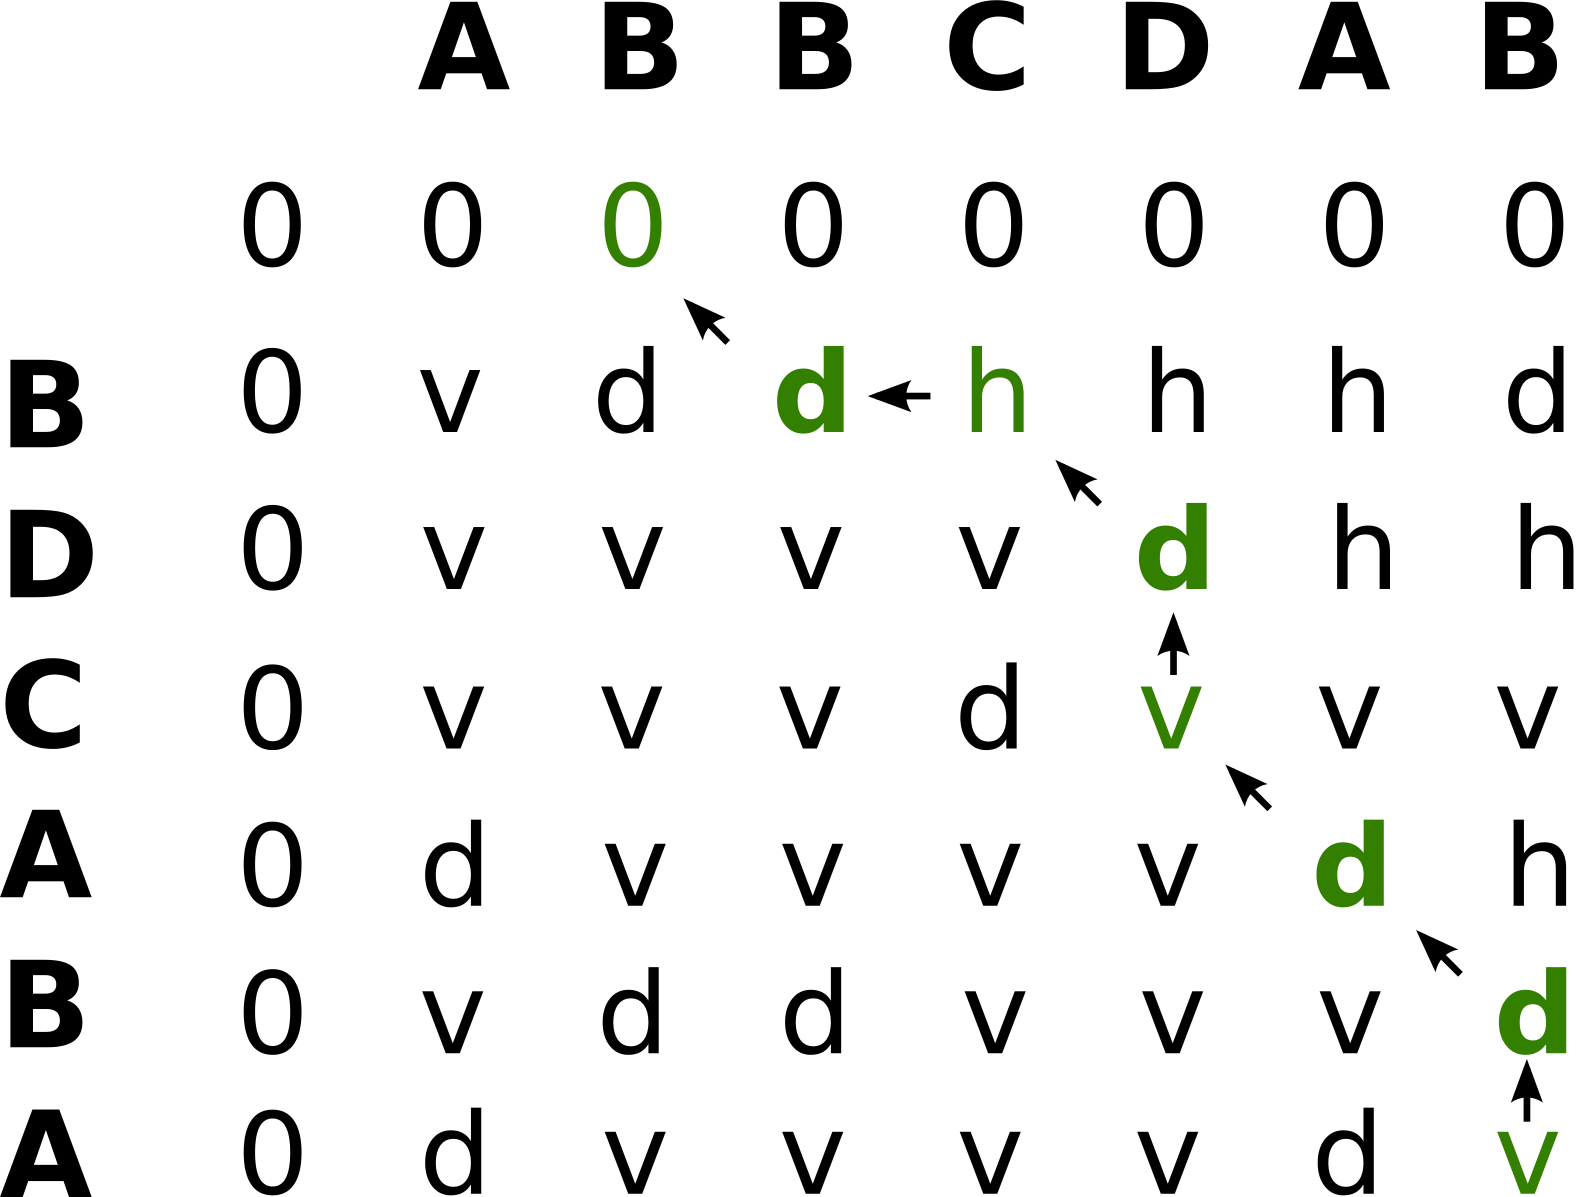
\includegraphics[width=0.75\linewidth]{images/lcstable10.png}
\end{center}
\end{frame}

\begin{frame}[fragile]
\frametitle{LCS} 
\begin{center}
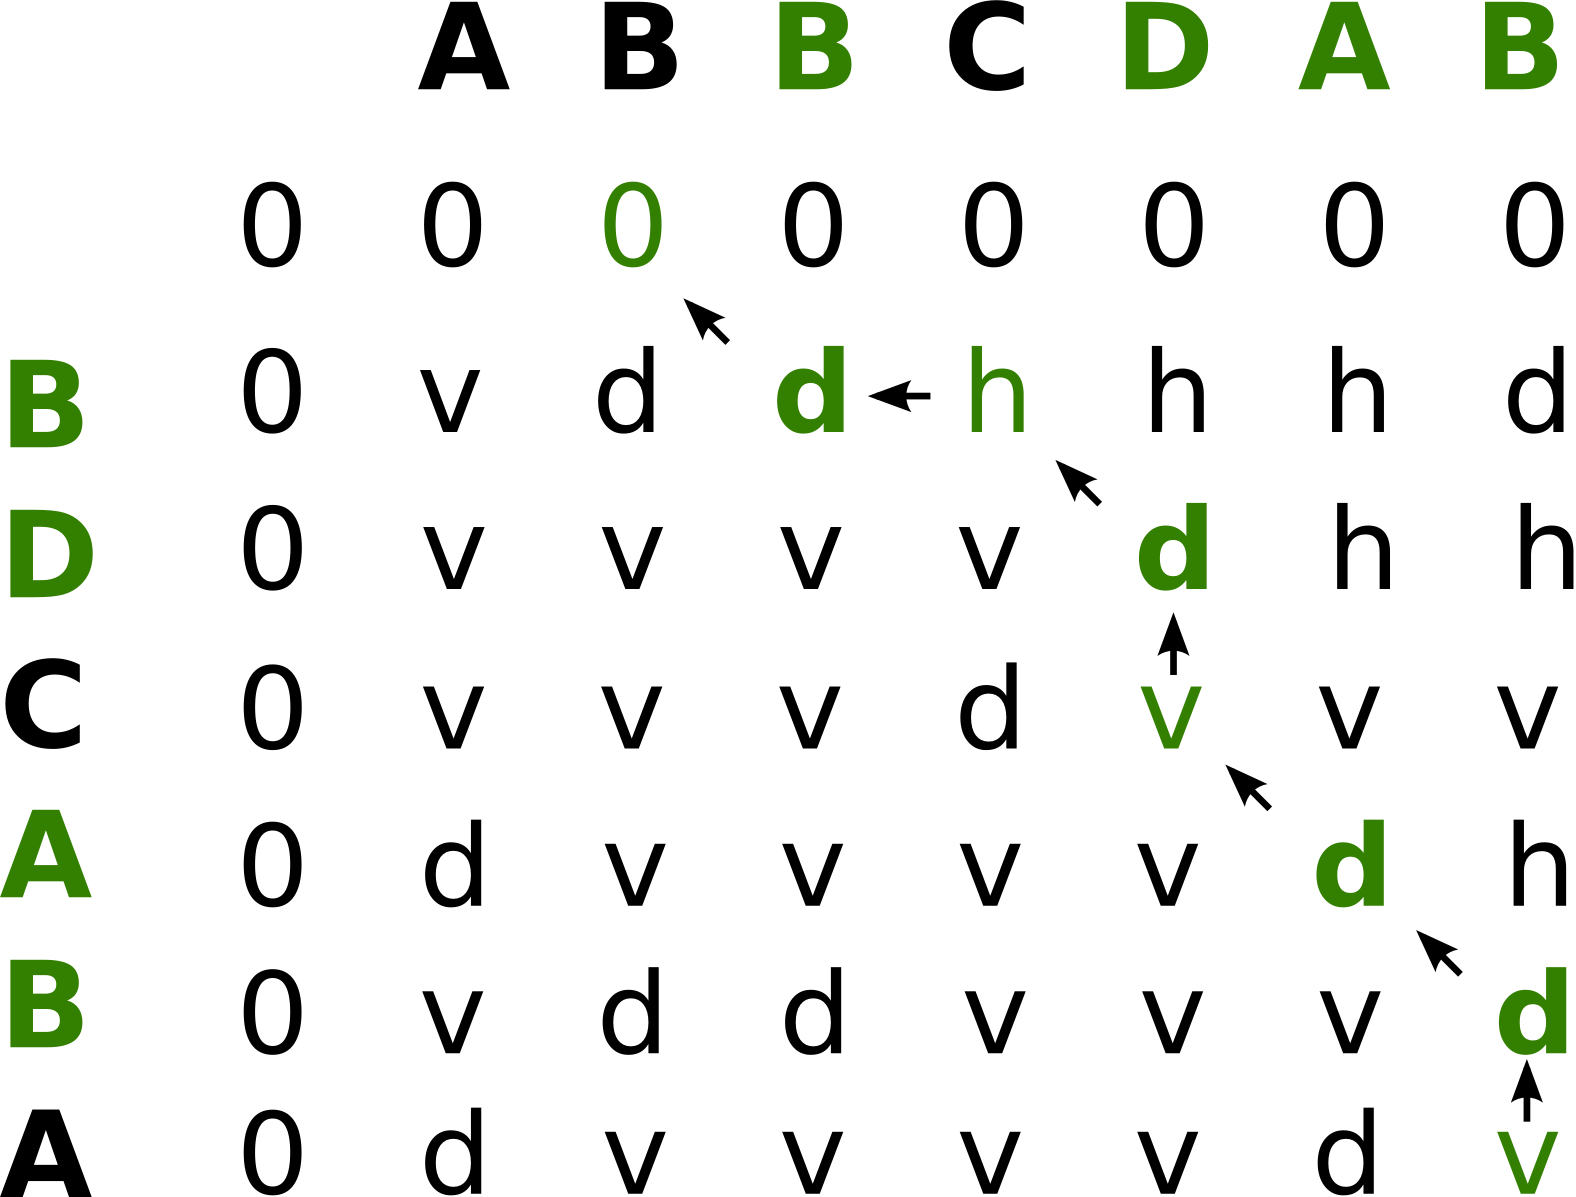
\includegraphics[width=0.75\linewidth]{images/lcstable11.png}
\end{center}
\end{frame}


\end{document}
